% Created by tikzDevice version 0.12.6 on 2025-04-02 09:32:19
% !TEX encoding = UTF-8 Unicode
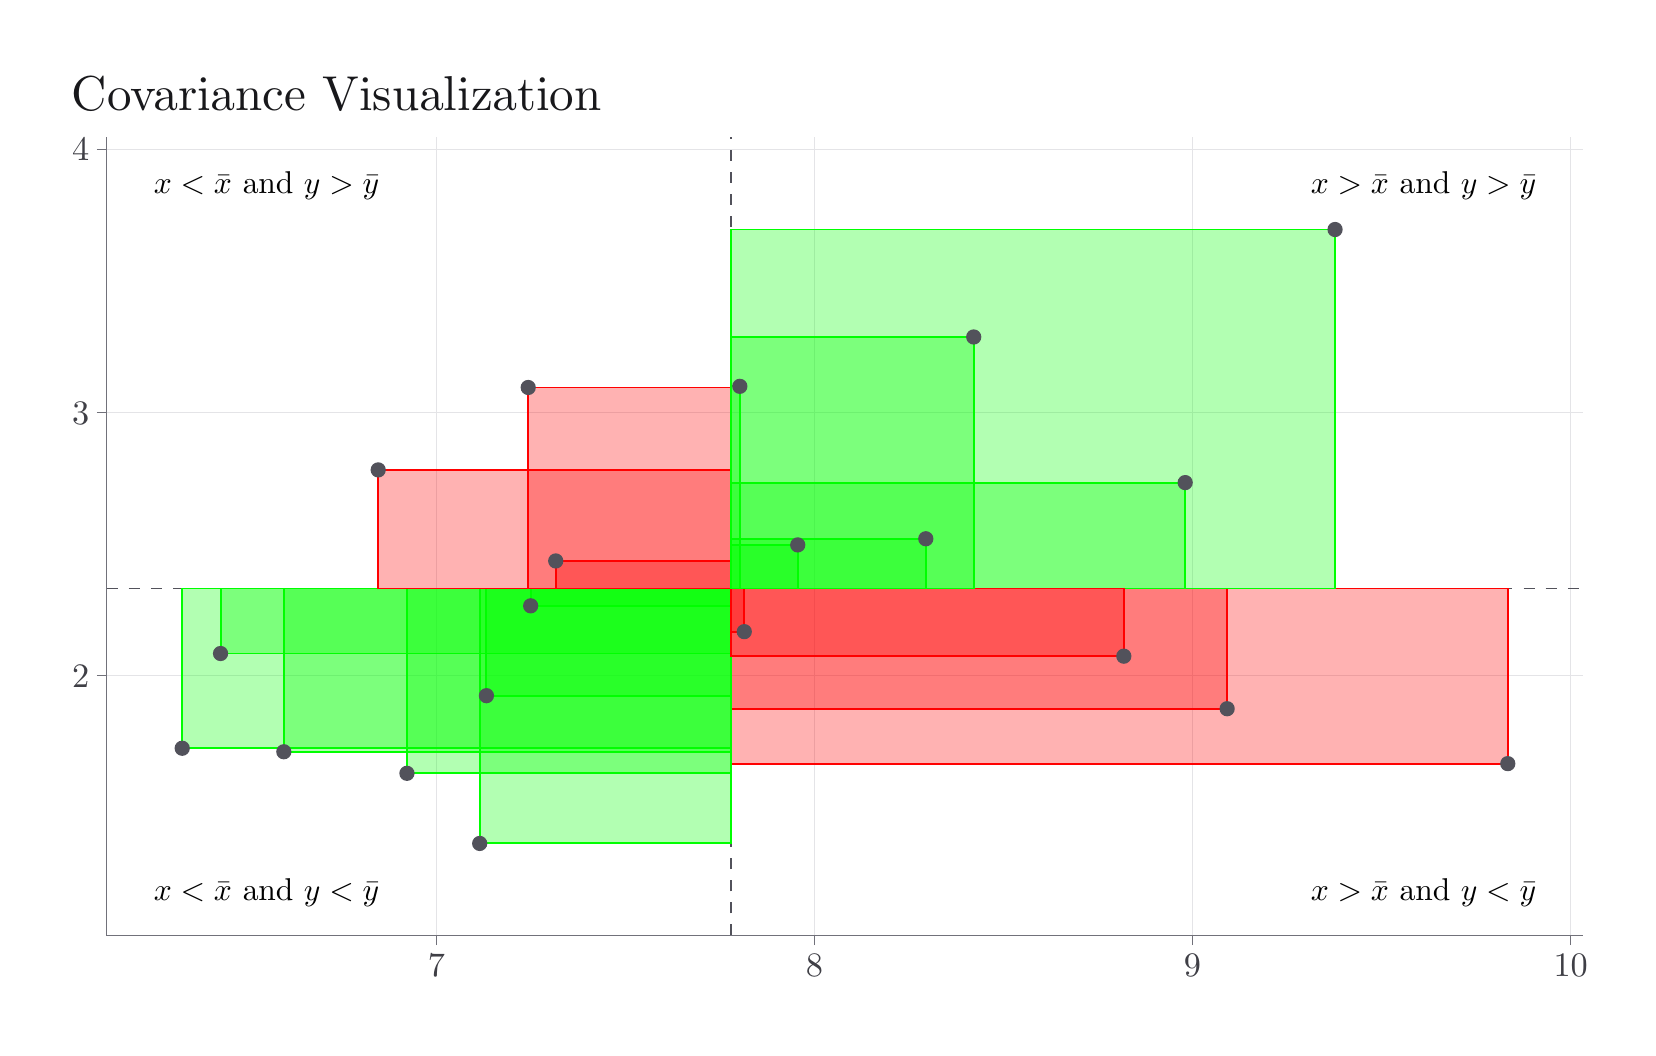
\begin{tikzpicture}[x=1pt,y=1pt]
\definecolor{fillColor}{RGB}{255,255,255}
\path[use as bounding box,fill=fillColor] (0,0) rectangle (578.16,361.35);
\begin{scope}
\path[clip] (  0.00,  0.00) rectangle (578.16,361.35);
\definecolor{drawColor}{RGB}{255,255,255}

\path[draw=drawColor,line width= 0.7pt,line join=round,line cap=round,fill=fillColor] (  0.00,  0.00) rectangle (578.16,361.35);
\end{scope}
\begin{scope}
\path[clip] ( 28.52, 33.29) rectangle (562.16,321.70);
\definecolor{drawColor}{RGB}{255,255,255}
\definecolor{fillColor}{RGB}{255,255,255}

\path[draw=drawColor,line width= 0.7pt,line join=round,line cap=round,fill=fillColor] ( 28.52, 33.29) rectangle (562.16,321.70);
\definecolor{drawColor}{RGB}{228,228,231}

\path[draw=drawColor,line width= 0.4pt,line join=round] ( 28.52,127.27) --
	(562.16,127.27);

\path[draw=drawColor,line width= 0.4pt,line join=round] ( 28.52,222.37) --
	(562.16,222.37);

\path[draw=drawColor,line width= 0.4pt,line join=round] ( 28.52,317.48) --
	(562.16,317.48);

\path[draw=drawColor,line width= 0.4pt,line join=round] (147.67, 33.29) --
	(147.67,321.70);

\path[draw=drawColor,line width= 0.4pt,line join=round] (284.30, 33.29) --
	(284.30,321.70);

\path[draw=drawColor,line width= 0.4pt,line join=round] (420.93, 33.29) --
	(420.93,321.70);

\path[draw=drawColor,line width= 0.4pt,line join=round] (557.57, 33.29) --
	(557.57,321.70);
\definecolor{drawColor}{RGB}{82,82,91}

\path[draw=drawColor,line width= 0.7pt,dash pattern=on 4pt off 4pt ,line join=round] ( 28.52,158.70) -- (562.16,158.70);

\path[draw=drawColor,line width= 0.7pt,dash pattern=on 4pt off 4pt ,line join=round] (254.01, 33.29) -- (254.01,321.70);
\definecolor{drawColor}{RGB}{255,0,0}
\definecolor{fillColor}{RGB}{255,0,0}

\path[draw=drawColor,line width= 0.7pt,fill=fillColor,fill opacity=0.30] (254.01,115.25) rectangle (433.42,158.70);
\definecolor{drawColor}{RGB}{0,255,0}
\definecolor{fillColor}{RGB}{0,255,0}

\path[draw=drawColor,line width= 0.7pt,fill=fillColor,fill opacity=0.30] ( 69.70,135.20) rectangle (254.01,158.70);
\definecolor{drawColor}{RGB}{255,0,0}
\definecolor{fillColor}{RGB}{255,0,0}

\path[draw=drawColor,line width= 0.7pt,fill=fillColor,fill opacity=0.30] (190.81,158.70) rectangle (254.01,168.65);
\definecolor{drawColor}{RGB}{0,255,0}
\definecolor{fillColor}{RGB}{0,255,0}

\path[draw=drawColor,line width= 0.7pt,fill=fillColor,fill opacity=0.30] (137.05, 91.91) rectangle (254.01,158.70);

\path[draw=drawColor,line width= 0.7pt,fill=fillColor,fill opacity=0.30] ( 55.84,100.97) rectangle (254.01,158.70);

\path[draw=drawColor,line width= 0.7pt,fill=fillColor,fill opacity=0.30] (254.01,158.70) rectangle (418.26,196.96);
\definecolor{drawColor}{RGB}{255,0,0}
\definecolor{fillColor}{RGB}{255,0,0}

\path[draw=drawColor,line width= 0.7pt,fill=fillColor,fill opacity=0.30] (254.01, 95.41) rectangle (534.83,158.70);
\definecolor{drawColor}{RGB}{0,255,0}
\definecolor{fillColor}{RGB}{0,255,0}

\path[draw=drawColor,line width= 0.7pt,fill=fillColor,fill opacity=0.30] (254.01,158.70) rectangle (472.42,288.41);

\path[draw=drawColor,line width= 0.7pt,fill=fillColor,fill opacity=0.30] (165.77,119.96) rectangle (254.01,158.70);

\path[draw=drawColor,line width= 0.7pt,fill=fillColor,fill opacity=0.30] ( 92.56, 99.70) rectangle (254.01,158.70);

\path[draw=drawColor,line width= 0.7pt,fill=fillColor,fill opacity=0.30] (163.34, 66.57) rectangle (254.01,158.70);
\definecolor{drawColor}{RGB}{255,0,0}
\definecolor{fillColor}{RGB}{255,0,0}

\path[draw=drawColor,line width= 0.7pt,fill=fillColor,fill opacity=0.30] (254.01,143.10) rectangle (258.94,158.70);
\definecolor{drawColor}{RGB}{0,255,0}
\definecolor{fillColor}{RGB}{0,255,0}

\path[draw=drawColor,line width= 0.7pt,fill=fillColor,fill opacity=0.30] (181.75,152.43) rectangle (254.01,158.70);
\definecolor{drawColor}{RGB}{255,0,0}
\definecolor{fillColor}{RGB}{255,0,0}

\path[draw=drawColor,line width= 0.7pt,fill=fillColor,fill opacity=0.30] (180.87,158.70) rectangle (254.01,231.33);

\path[draw=drawColor,line width= 0.7pt,fill=fillColor,fill opacity=0.30] (126.66,158.70) rectangle (254.01,201.55);

\path[draw=drawColor,line width= 0.7pt,fill=fillColor,fill opacity=0.30] (254.01,134.24) rectangle (396.09,158.70);
\definecolor{drawColor}{RGB}{0,255,0}
\definecolor{fillColor}{RGB}{0,255,0}

\path[draw=drawColor,line width= 0.7pt,fill=fillColor,fill opacity=0.30] (254.01,158.70) rectangle (257.34,231.74);

\path[draw=drawColor,line width= 0.7pt,fill=fillColor,fill opacity=0.30] (254.01,158.70) rectangle (278.26,174.44);

\path[draw=drawColor,line width= 0.7pt,fill=fillColor,fill opacity=0.30] (254.01,158.70) rectangle (324.53,176.66);

\path[draw=drawColor,line width= 0.7pt,fill=fillColor,fill opacity=0.30] (254.01,158.70) rectangle (341.85,249.58);
\definecolor{drawColor}{RGB}{82,82,91}
\definecolor{fillColor}{RGB}{82,82,91}

\path[draw=drawColor,line width= 0.5pt,line join=round,line cap=round,fill=fillColor] (433.42,115.25) circle (  2.50);

\path[draw=drawColor,line width= 0.5pt,line join=round,line cap=round,fill=fillColor] ( 69.70,135.20) circle (  2.50);

\path[draw=drawColor,line width= 0.5pt,line join=round,line cap=round,fill=fillColor] (190.81,168.65) circle (  2.50);

\path[draw=drawColor,line width= 0.5pt,line join=round,line cap=round,fill=fillColor] (137.05, 91.91) circle (  2.50);

\path[draw=drawColor,line width= 0.5pt,line join=round,line cap=round,fill=fillColor] ( 55.84,100.97) circle (  2.50);

\path[draw=drawColor,line width= 0.5pt,line join=round,line cap=round,fill=fillColor] (418.26,196.96) circle (  2.50);

\path[draw=drawColor,line width= 0.5pt,line join=round,line cap=round,fill=fillColor] (534.83, 95.41) circle (  2.50);

\path[draw=drawColor,line width= 0.5pt,line join=round,line cap=round,fill=fillColor] (472.42,288.41) circle (  2.50);

\path[draw=drawColor,line width= 0.5pt,line join=round,line cap=round,fill=fillColor] (165.77,119.96) circle (  2.50);

\path[draw=drawColor,line width= 0.5pt,line join=round,line cap=round,fill=fillColor] ( 92.56, 99.70) circle (  2.50);

\path[draw=drawColor,line width= 0.5pt,line join=round,line cap=round,fill=fillColor] (163.34, 66.57) circle (  2.50);

\path[draw=drawColor,line width= 0.5pt,line join=round,line cap=round,fill=fillColor] (258.94,143.10) circle (  2.50);

\path[draw=drawColor,line width= 0.5pt,line join=round,line cap=round,fill=fillColor] (181.75,152.43) circle (  2.50);

\path[draw=drawColor,line width= 0.5pt,line join=round,line cap=round,fill=fillColor] (180.87,231.33) circle (  2.50);

\path[draw=drawColor,line width= 0.5pt,line join=round,line cap=round,fill=fillColor] (126.66,201.55) circle (  2.50);

\path[draw=drawColor,line width= 0.5pt,line join=round,line cap=round,fill=fillColor] (396.09,134.24) circle (  2.50);

\path[draw=drawColor,line width= 0.5pt,line join=round,line cap=round,fill=fillColor] (257.34,231.74) circle (  2.50);

\path[draw=drawColor,line width= 0.5pt,line join=round,line cap=round,fill=fillColor] (278.26,174.44) circle (  2.50);

\path[draw=drawColor,line width= 0.5pt,line join=round,line cap=round,fill=fillColor] (324.53,176.66) circle (  2.50);

\path[draw=drawColor,line width= 0.5pt,line join=round,line cap=round,fill=fillColor] (341.85,249.58) circle (  2.50);
\definecolor{fillColor}{RGB}{255,255,255}

\path[fill=fillColor] (462.45,297.93) --
	(546.44,297.93) --
	(546.36,297.93) --
	(546.69,297.94) --
	(547.01,298.01) --
	(547.32,298.12) --
	(547.61,298.29) --
	(547.86,298.50) --
	(548.08,298.75) --
	(548.26,299.03) --
	(548.39,299.33) --
	(548.47,299.65) --
	(548.50,299.98) --
	(548.50,299.98) --
	(548.50,310.56) --
	(548.50,310.56) --
	(548.47,310.89) --
	(548.39,311.21) --
	(548.26,311.52) --
	(548.08,311.80) --
	(547.86,312.04) --
	(547.61,312.25) --
	(547.32,312.42) --
	(547.01,312.54) --
	(546.69,312.60) --
	(546.44,312.62) --
	(462.45,312.62) --
	(462.70,312.60) --
	(462.37,312.62) --
	(462.04,312.58) --
	(461.73,312.48) --
	(461.43,312.34) --
	(461.15,312.15) --
	(460.92,311.92) --
	(460.72,311.66) --
	(460.56,311.37) --
	(460.46,311.05) --
	(460.40,310.73) --
	(460.40,310.56) --
	(460.40,299.98) --
	(460.40,300.15) --
	(460.40,299.82) --
	(460.46,299.49) --
	(460.56,299.18) --
	(460.72,298.88) --
	(460.92,298.62) --
	(461.15,298.39) --
	(461.43,298.20) --
	(461.73,298.06) --
	(462.04,297.97) --
	(462.37,297.93) --
	cycle;
\end{scope}
\begin{scope}
\path[clip] ( 28.52, 33.29) rectangle (562.16,321.70);
\definecolor{drawColor}{RGB}{0,0,0}

\node[text=drawColor,anchor=base east,inner sep=0pt, outer sep=0pt, scale=  1.14] at (545.07,301.35) {$x > \bar{x}$ and $y > \bar{y}$};
\end{scope}
\begin{scope}
\path[clip] ( 28.52, 33.29) rectangle (562.16,321.70);
\definecolor{fillColor}{RGB}{255,255,255}

\path[fill=fillColor] ( 44.24, 42.37) --
	(128.22, 42.37) --
	(128.14, 42.37) --
	(128.47, 42.39) --
	(128.80, 42.45) --
	(129.11, 42.57) --
	(129.39, 42.73) --
	(129.65, 42.94) --
	(129.87, 43.19) --
	(130.05, 43.47) --
	(130.17, 43.78) --
	(130.25, 44.10) --
	(130.28, 44.43) --
	(130.28, 44.43) --
	(130.28, 55.01) --
	(130.28, 55.01) --
	(130.25, 55.34) --
	(130.17, 55.66) --
	(130.05, 55.96) --
	(129.87, 56.24) --
	(129.65, 56.49) --
	(129.39, 56.70) --
	(129.11, 56.86) --
	(128.80, 56.98) --
	(128.47, 57.05) --
	(128.22, 57.06) --
	( 44.24, 57.06) --
	( 44.49, 57.05) --
	( 44.16, 57.06) --
	( 43.83, 57.02) --
	( 43.51, 56.93) --
	( 43.21, 56.79) --
	( 42.94, 56.60) --
	( 42.70, 56.37) --
	( 42.50, 56.10) --
	( 42.35, 55.81) --
	( 42.24, 55.50) --
	( 42.19, 55.17) --
	( 42.18, 55.01) --
	( 42.18, 44.43) --
	( 42.19, 44.59) --
	( 42.19, 44.26) --
	( 42.24, 43.93) --
	( 42.35, 43.62) --
	( 42.50, 43.33) --
	( 42.70, 43.06) --
	( 42.94, 42.83) --
	( 43.21, 42.65) --
	( 43.51, 42.50) --
	( 43.83, 42.41) --
	( 44.16, 42.37) --
	cycle;
\end{scope}
\begin{scope}
\path[clip] ( 28.52, 33.29) rectangle (562.16,321.70);
\definecolor{drawColor}{RGB}{0,0,0}

\node[text=drawColor,anchor=base west,inner sep=0pt, outer sep=0pt, scale=  1.14] at ( 45.61, 45.80) {$x < \bar{x}$ and $y < \bar{y}$};
\end{scope}
\begin{scope}
\path[clip] ( 28.52, 33.29) rectangle (562.16,321.70);
\definecolor{fillColor}{RGB}{255,255,255}

\path[fill=fillColor] (462.45, 42.37) --
	(546.44, 42.37) --
	(546.36, 42.37) --
	(546.69, 42.39) --
	(547.01, 42.45) --
	(547.32, 42.57) --
	(547.61, 42.73) --
	(547.86, 42.94) --
	(548.08, 43.19) --
	(548.26, 43.47) --
	(548.39, 43.78) --
	(548.47, 44.10) --
	(548.50, 44.43) --
	(548.50, 44.43) --
	(548.50, 55.01) --
	(548.50, 55.01) --
	(548.47, 55.34) --
	(548.39, 55.66) --
	(548.26, 55.96) --
	(548.08, 56.24) --
	(547.86, 56.49) --
	(547.61, 56.70) --
	(547.32, 56.86) --
	(547.01, 56.98) --
	(546.69, 57.05) --
	(546.44, 57.06) --
	(462.45, 57.06) --
	(462.70, 57.05) --
	(462.37, 57.06) --
	(462.04, 57.02) --
	(461.73, 56.93) --
	(461.43, 56.79) --
	(461.15, 56.60) --
	(460.92, 56.37) --
	(460.72, 56.10) --
	(460.56, 55.81) --
	(460.46, 55.50) --
	(460.40, 55.17) --
	(460.40, 55.01) --
	(460.40, 44.43) --
	(460.40, 44.59) --
	(460.40, 44.26) --
	(460.46, 43.93) --
	(460.56, 43.62) --
	(460.72, 43.33) --
	(460.92, 43.06) --
	(461.15, 42.83) --
	(461.43, 42.65) --
	(461.73, 42.50) --
	(462.04, 42.41) --
	(462.37, 42.37) --
	cycle;
\end{scope}
\begin{scope}
\path[clip] ( 28.52, 33.29) rectangle (562.16,321.70);
\definecolor{drawColor}{RGB}{0,0,0}

\node[text=drawColor,anchor=base east,inner sep=0pt, outer sep=0pt, scale=  1.14] at (545.07, 45.80) {$x > \bar{x}$ and $y < \bar{y}$};
\end{scope}
\begin{scope}
\path[clip] ( 28.52, 33.29) rectangle (562.16,321.70);
\definecolor{fillColor}{RGB}{255,255,255}

\path[fill=fillColor] ( 44.24,297.93) --
	(128.22,297.93) --
	(128.14,297.93) --
	(128.47,297.94) --
	(128.80,298.01) --
	(129.11,298.12) --
	(129.39,298.29) --
	(129.65,298.50) --
	(129.87,298.75) --
	(130.05,299.03) --
	(130.17,299.33) --
	(130.25,299.65) --
	(130.28,299.98) --
	(130.28,299.98) --
	(130.28,310.56) --
	(130.28,310.56) --
	(130.25,310.89) --
	(130.17,311.21) --
	(130.05,311.52) --
	(129.87,311.80) --
	(129.65,312.04) --
	(129.39,312.25) --
	(129.11,312.42) --
	(128.80,312.54) --
	(128.47,312.60) --
	(128.22,312.62) --
	( 44.24,312.62) --
	( 44.49,312.60) --
	( 44.16,312.62) --
	( 43.83,312.58) --
	( 43.51,312.48) --
	( 43.21,312.34) --
	( 42.94,312.15) --
	( 42.70,311.92) --
	( 42.50,311.66) --
	( 42.35,311.37) --
	( 42.24,311.05) --
	( 42.19,310.73) --
	( 42.18,310.56) --
	( 42.18,299.98) --
	( 42.19,300.15) --
	( 42.19,299.82) --
	( 42.24,299.49) --
	( 42.35,299.18) --
	( 42.50,298.88) --
	( 42.70,298.62) --
	( 42.94,298.39) --
	( 43.21,298.20) --
	( 43.51,298.06) --
	( 43.83,297.97) --
	( 44.16,297.93) --
	cycle;
\end{scope}
\begin{scope}
\path[clip] ( 28.52, 33.29) rectangle (562.16,321.70);
\definecolor{drawColor}{RGB}{0,0,0}

\node[text=drawColor,anchor=base west,inner sep=0pt, outer sep=0pt, scale=  1.14] at ( 45.61,301.35) {$x < \bar{x}$ and $y > \bar{y}$};
\end{scope}
\begin{scope}
\path[clip] (  0.00,  0.00) rectangle (578.16,361.35);
\definecolor{drawColor}{RGB}{113,113,122}

\path[draw=drawColor,line width= 0.3pt,line join=round] ( 28.52, 33.29) --
	( 28.52,321.70);
\end{scope}
\begin{scope}
\path[clip] (  0.00,  0.00) rectangle (578.16,361.35);
\definecolor{drawColor}{RGB}{63,63,70}

\node[text=drawColor,anchor=base east,inner sep=0pt, outer sep=0pt, scale=  1.24] at ( 22.22,122.98) {2};

\node[text=drawColor,anchor=base east,inner sep=0pt, outer sep=0pt, scale=  1.24] at ( 22.22,218.09) {3};

\node[text=drawColor,anchor=base east,inner sep=0pt, outer sep=0pt, scale=  1.24] at ( 22.22,313.19) {4};
\end{scope}
\begin{scope}
\path[clip] (  0.00,  0.00) rectangle (578.16,361.35);
\definecolor{drawColor}{RGB}{113,113,122}

\path[draw=drawColor,line width= 0.3pt,line join=round] ( 25.02,127.27) --
	( 28.52,127.27);

\path[draw=drawColor,line width= 0.3pt,line join=round] ( 25.02,222.37) --
	( 28.52,222.37);

\path[draw=drawColor,line width= 0.3pt,line join=round] ( 25.02,317.48) --
	( 28.52,317.48);
\end{scope}
\begin{scope}
\path[clip] (  0.00,  0.00) rectangle (578.16,361.35);
\definecolor{drawColor}{RGB}{113,113,122}

\path[draw=drawColor,line width= 0.3pt,line join=round] ( 28.52, 33.29) --
	(562.16, 33.29);
\end{scope}
\begin{scope}
\path[clip] (  0.00,  0.00) rectangle (578.16,361.35);
\definecolor{drawColor}{RGB}{113,113,122}

\path[draw=drawColor,line width= 0.3pt,line join=round] (147.67, 29.79) --
	(147.67, 33.29);

\path[draw=drawColor,line width= 0.3pt,line join=round] (284.30, 29.79) --
	(284.30, 33.29);

\path[draw=drawColor,line width= 0.3pt,line join=round] (420.93, 29.79) --
	(420.93, 33.29);

\path[draw=drawColor,line width= 0.3pt,line join=round] (557.57, 29.79) --
	(557.57, 33.29);
\end{scope}
\begin{scope}
\path[clip] (  0.00,  0.00) rectangle (578.16,361.35);
\definecolor{drawColor}{RGB}{63,63,70}

\node[text=drawColor,anchor=base,inner sep=0pt, outer sep=0pt, scale=  1.24] at (147.67, 18.42) {7};

\node[text=drawColor,anchor=base,inner sep=0pt, outer sep=0pt, scale=  1.24] at (284.30, 18.42) {8};

\node[text=drawColor,anchor=base,inner sep=0pt, outer sep=0pt, scale=  1.24] at (420.93, 18.42) {9};

\node[text=drawColor,anchor=base,inner sep=0pt, outer sep=0pt, scale=  1.24] at (557.57, 18.42) {10};
\end{scope}
\begin{scope}
\path[clip] (  0.00,  0.00) rectangle (578.16,361.35);
\definecolor{drawColor}{RGB}{24,24,27}

\node[text=drawColor,anchor=base west,inner sep=0pt, outer sep=0pt, scale=  1.77] at ( 16.00,331.42) {Covariance Visualization};
\end{scope}
\end{tikzpicture}
